\documentclass[conference,a4paper]{IEEEtran}
% Native A4 conference option; original class, standard body font and spacing.
\usepackage{fontspec}
\setmainfont{texgyretermes-regular.otf}[BoldFont=texgyretermes-bold.otf,ItalicFont=texgyretermes-italic.otf,BoldItalicFont=texgyretermes-bolditalic.otf]
\usepackage{cite,amsmath,amssymb,graphicx,booktabs,url,array}
\usepackage[hidelinks]{hyperref}
\newcommand{\RescueTen}{533}
\newcommand{\RescueTwenty}{118}
\newcommand{\OffTwenty}{28.121}
\newcommand{\FullTwenty}{24.320}
\newcommand{\ModeReductionTwenty}{13.5}
\newcommand{\CollectedPairsTwenty}{235}
\newcommand{\CollectionsTwenty}{277}
\newcommand{\CpuChoice}{BiWFA with 20 threads in original order}
\newcommand{\SmallEGuard}{32.333}
\newcommand{\SmallEFull}{31.725}

\AtBeginDocument{\special{pdf:docinfo << /Title (Exact GPU Traceback under a Memory Budget: Reclamation and Worker Configuration) /Author (Dabin Jeong) >>}}
\begin{document}
\title{Exact GPU Traceback under a Memory Budget:\\Reclamation and Worker Configuration}
\author{\IEEEauthorblockN{Dabin Jeong}\IEEEauthorblockA{\textit{Korea University}\\cudabinary@korea.ac.kr}}
\maketitle
\begin{abstract}
Exact sequence alignment must return an optimal operation sequence as well as its score. In a persistent GPU implementation, reserving traceback history per worker couples memory capacity to the worker pool and can trigger CPU recomputation. We adapt existing WFA2 reachability garbage collection (GC) to block-local WFA-GPU arenas, independently controlling arena capacity and the wavefront execution bound. On an RTX 4060 Ti, we compare complete jobs under tracked CUDA reservation caps, including CPU routing, rescue, synchronization, and full CIGAR output. For 10,000 public Oxford Nanopore Technologies (ONT) pairs, matched small-arena controls show that collection prevents capacity rescues and reduces completion time; the same-binary 20M/32 ablation reduces the median by \ModeReductionTwenty{} percent and rescues from 118 to zero, confirming the effect without changing its allocated workspace or register configuration. Measured generation, retained ancestor closure, and completion events explain how append space is reused. Stronger software controls delimit the result: smaller execution bounds increase CPU rescue, while CPU BiWFA remains competitive on long ONT and faster in refreshed short-ONT and circular consensus sequencing (CCS) comparisons. The contribution is a qualified GPU implementation and a measured operating region for exact traceback, rather than a new reclamation principle or a universal GPU advantage.
\end{abstract}
\begin{IEEEkeywords}sequence alignment, exact traceback, wavefront, memory reclamation, GPU\end{IEEEkeywords}

\section{Introduction}
The wavefront alignment algorithm (WFA) advances furthest-reaching states at increasing alignment costs, avoiding much of the dynamic-programming matrix for similar sequences \cite{wfa2021}. Computing an optimal score and returning a full alignment operation sequence, conventionally represented by a CIGAR string, are different computational contracts. Rolling wavefronts suffice for score computation, whereas traceback requires retaining or reconstructing history. Score-only timing and storage therefore do not establish the cost of producing an exact alignment.

WFA-GPU assigns independent pairs to persistent workers, each owning an append-only traceback arena \cite{wfagpu2023}. A large reservation protects difficult pairs but limits the worker pool under a memory cap. A smaller arena permits more workers, at the cost of possible CPU realignment or reclamation. More workers can also compete for resources. The useful objective is consequently whole-job completion under an explicit resource budget, rather than arena bytes, nominal concurrency, or kernel throughput in isolation.

This tradeoff is already recognized in prior characterization \cite{characterisation2026}. The open question we address is narrower: \emph{Can active-root collection make a small worker arena useful for exact full-CIGAR jobs after simple no-GC, execution-bound, and CPU alternatives are allowed?} We separate the wavefront execution bound $E$, arena capacity $C$, and worker count $w$, and apply the existing WFA2 mark/compact principle \cite{wfa2lib2026}. Collection is a concrete way of changing feasible execution points; it is not assumed to reduce the recurrence work.

Our contributions are threefold. First, we implement guarded capacity and block-local, in-place reachability collection with consistent root/predecessor remapping in a full-traceback GPU path. Second, matched $C,w$ controls, including GC on/off in the same binary, connect reclaimed space to avoided CPU recomputation and whole-job completion. Third, source-qualified root preservation, actual compactor boundary tests, measured generation/retention, and byte-level allocation receipts make the tested mechanism reproducible. We attribute the GC principle, persistent scheduling, and exact CPU rescue to existing software. A selector is not part of the method.

\section{Contract and Representation}
\subsection{Exact Output and Supported Execution}
Every comparison requires exact global gap-affine alignment with match cost zero, mismatch cost two, and gap cost $3+L$ for length $L$, without heuristics or banding. Validation checks the reference optimum, positive-length full run-length-encoded CIGAR, actual matching/mismatching bases, affine insertion/deletion cost, and complete consumption of both sequences. Different CIGAR strings for tied optimal paths are accepted. The independent small-input reference uses affine dynamic programming; public inputs use frozen optimal-score references with the same scoring contract.

The GPU implementation uses signed 16-bit offsets and accepts A/C/G/T pairs with both lengths below 32,768. Unsupported lengths or characters retain their original pairing and are CPU-routed. The configured $E$ bounds GPU execution; it is not an optimum score known before alignment. Exhausting that bound or an arena invokes exact CPU rescue, so changing $E$ can change execution without changing the final contract. We record support routing, execution-bound failure, arena failure, collector/chain error, and device-allocation failure separately. ``GPU-completed'' excludes CPU realignment but still includes CPU RLE reconstruction and output.

\subsection{Arena Occupancy, Generation, and Liveness}
An offloaded traceback record contains a compressed operation vector and a predecessor index, totaling eight bytes. Index zero is NULL. The next append position $H$ starts at one; $H-1$ is current occupied storage. After collection it decreases, and must not be called cumulative generation. A wavefront stores both a partial operation vector not yet offloaded and a pointer to its older chain. Valid stored pointers form roots; their ancestor closure is the collector's retained set. That set is conservative, not an algorithm-independent lower bound on required memory.

A worker is a persistent CUDA block with a private arena. The configured pool $w$ is distinct from simultaneously resident blocks, which we do not infer from $w$. Batch size $B$ determines input/result buffering and is also distinct. The original arena bound is
\begin{equation} C_{\rm src}=(2E+1)\lfloor E/8\rfloor.\label{eq:bound}\end{equation}
The guarded path instead uses $C=\min(C_{\rm requested},C_{\rm src})$. Appends check capacity before storing; failures are reported at the common score boundary and rescued exactly. This separates traceback capacity from the GPU execution limit.

\section{Block-Local Traceback Reclamation}
\subsection{Collection and In-Place Relocation}
Full GC starts at a synchronized score boundary when $H$ reaches an initial trigger $3C/4$. Startup leaves conservative headroom $R=3(2E+1)$ for a following update. After collection, the next trigger is
\begin{equation}\tau' = \min(C-R,\max(3C/4,H'+C/16)).\end{equation}
The implementation checks whether the retained set plus headroom fits; an invariant or final-chain error disqualifies the run even if a library fallback produces output.

Each worker clears its bitmap and marks the ancestors of all valid pointers in existing $M/I/D$ wavefronts across five rolling slots. Backward predecessors allow a traversal to stop at an already marked ancestor; the phase barrier ensures all such traversals finish before rank/remapping. An exclusive scan of popcounts gives the number of marked records preceding each 32-record word. The word rank plus the inclusive bit popcount maps a live record $i$ to $f(i)$, with NULL mapped separately to zero.

Stable rank is injective on live records and satisfies $f(i)\leq i$. Threads visit ascending 256-record tiles, load live payloads and predecessor indices into registers, synchronize, store at remapped destinations with remapped links, and synchronize again. Because destinations cannot exceed source indices, a store cannot damage an unread source in a later tile. Active roots are remapped with the same function; pointers at invalid offsets are cleared. The append position becomes $H'=|\mathcal L|+1$. No second full-size relocation arena is reserved. Other workers use disjoint arenas and scratch. Collection pauses recurrence only within its worker.

\subsection{Connecting Preservation Conditions to Code}
\textbf{Root-closure condition.} For the fixed penalties, recurrence at score $s$ reads $M_{s-2}$, $M_{s-4}$ and $I/D_{s-1}$. At the collection boundary, five rolling slots represent ages zero through four. Keeping every valid $M/I/D$ pointer in those slots includes the states from which future recurrence can obtain pointers. The collector moves offloaded records and remaps their stored roots; partial vectors remain in the wavefront arrays. Per-diagonal temporary pointers used during recurrence are finished before the existing block barrier; subsequent recurrence loads remapped pointers. This is a code-specific dependency argument for the tested penalties, not a claim for arbitrary penalties or asynchronous collection.

\begin{table}[t]
\caption{References Preserved at the Collection Boundary}
\label{tab:roots}\centering
\begin{tabular}{>{\raggedright\arraybackslash}p{.28\columnwidth}>{\raggedright\arraybackslash}p{.61\columnwidth}}\toprule
Reference & Representation and preservation\\\midrule
Rolling $M/I/D$ & Valid pointers across five slots; mark and remap.\\
Offloaded records & Immutable payload and older predecessor; mark closure and remap links.\\
Partial vectors & Stored with wavefront state; unchanged by compaction.\\
Recurrence temporaries & Quiescent at the preceding block barrier; reloaded next update.\\
Final extraction & Runs after collection; follows the remapped chain.\\\bottomrule
\end{tabular}
\end{table}

The revised common kernel designates thread zero to initialize the append cursor and invalidate two shared wavefront-metadata groups. The existing dominating barriers remain; thread-local distance, steps, and rolling indices continue to advance on every thread. Both guarded and GC binaries receive the same fixes. A source audit and finite validation do not establish universal CUDA race freedom. Compute Sanitizer~\cite{sanitizer2026} could not initialize the WDDM debugger interface in this WSL environment; its setup errors are retained, including a memcheck exit code zero that still reported errors.

Validation separates three questions. Independent affine DP checks 160 short pairs in each alignment path; they complete on the GPU but invoke no collection. Actual-helper tests cover 33 single-worker DAG cases with two consecutive collections, then 96 worker cases in two-block launches with three collections including append-after-remap. They include NULL/shared ancestry and record boundaries 31/32/33, 255/256/257 and 8,191/8,192/8,193. Public-input diagnostics then check repeated actual collection and optimal full CIGAR, complementing those unit tests.

\subsection{Reservation and Diagnostic Accounting}
Tracked arena and GC scratch are
\begin{equation}M_{\rm arena}=8Cw,\qquad M_{\rm GC}=8w\lceil C/32\rceil.\label{eq:memory}\end{equation}
The scratch consists of four-byte bitmap words and four-byte ranks, or 3.125\% of arena storage for these capacities. It remains allocated in the same-binary GC-off control and is absent from the lighter guarded binary. Rolling wavefronts, result buffers, input packing, metadata, status, and padding are also counted. The executable integer-byte formula and per-run allocation receipts are in the named supplementary material. Logical collection reuses the reserved arena; it does not return that allocation to CUDA.

Tracked CUDA API reservation excludes driver/context/module internals, host/pinned memory and physical VRAM residency or paging. A reservation cap is therefore not a measurement of physical device occupancy. At $E=16,384$, \eqref{eq:bound} gives 67,110,912 records, or 512.016 MiB per worker, as a calculated bound rather than observed liveness.

Detailed diagnostics use a separate binary and extra trace storage. A successful cumulative-append counter adds increases in occupied storage at synchronized score boundaries and resets its previous-occupancy baseline after each collection. Its final value must equal final occupied records plus all reclaimed records. This identity checks accounting, not a free future-capacity predictor. Live counts are observed at collections; we do not claim a continuously measured live maximum. Worker cycles and overlapping spans are never summed into application wall-time fractions.

\section{Evaluation Method}
\subsection{Platform, Inputs, and Fixed Boundaries}
The platform is an RTX 4060 Ti (8,188 MiB) with a Core i5-14500, Ubuntu 26.04 under Windows Subsystem for Linux (WSL), 20 logical CPUs and approximately 15.5 GiB host RAM. We use driver 610.88, CUDA 13.3 and GCC 14. The source bases are WFA-GPU \texttt{ff981ad0}, current WFA2 \texttt{6176f947} and Singletrack \texttt{7185195}. Official upstream HEADs were checked on October 19, 2026; full hashes, modifications, commands and binaries are preserved. Metadata initialization, padding/size fixes, buffer reuse, removal of unnecessary arena clears, and current exact CPU rescue are shared baseline improvements.

The main input is the block-aligner v0.0.0 public file named ``50k'', with its original 10,000 ONT pairings.\footnote{\url{https://github.com/Daniel-Liu-c0deb0t/block-aligner/releases/tag/v0.0.0}} Maximum-sequence-length median is 6,104~bp, 90th percentile 31,352~bp and maximum 49,993~bp; pairs are not uniformly 50~kbp. Length support routes 888 pairs to the CPU; 9,112 are GPU-eligible. The old selection split alone chooses CPU/E candidates. The previously viewed confirmation split is not a new holdout. The shorter 4,488-pair ONT set excludes the initial 512 tuning pairs, and the entire 5,000-pair 10k file also occurs in the 50k file.

Independent-source CCS results use 2,375 confirmation pairs from \texttt{rw\_ccs.seq} in Zenodo 23118370 \cite{wfaCharacterization2026}: 2,365 GPU-eligible and ten character-unsupported pairs. Content-group splitting preceded inspection, and no pair duplicates were found against ONT. These are mapped public read--reference benchmarks, not an application arrival or concurrency trace. The original records are preserved. After the common-kernel change, the old fixed short/CCS settings are refreshed in three crossed runs each, without retuning or a fresh-holdout claim.

\subsection{Controls and Measurement Scope}
The mechanism controls fix $E=16,384 $, 256 threads/block and $B=512$, with decreasing maximum-length order and pair-ID tie breaking. We test guarded 10M/34 and 20M/32, their Full counterparts, and no-GC 10M/35 and 20M/33 where the allocation model fits the same 3/5.5~GiB caps. M means $2^{20}$ records. Same-binary mode 0/1 controls hold $C,w$, workspace and compiled resource requirements fixed; the lighter guarded build remains a primary baseline. Cross-binary differences include register/code effects and are not pure collection overhead.

Practical alternatives receive two smaller $E$ candidates, 4,096/8,192, per GPU family on selection data. Their fixed worker settings are bounded tests, not an exhaustive optimum. CPU screening includes current WFA2 high/med/low/ultralow modes, a descending-length control, and current Singletrack. A 12~GiB process address-space cap protects the host; RSS is recorded separately. Non-completing configurations are not scored as fast results. Supported GPU work uses four rescue threads concurrent with 16 unsupported-routing threads. CPU-only timing uses the selected feasible mode/thread/order; selection and its limitations are reported in the supplement.

Whole-job time begins after common config/reference/ID loading and includes actual input reading, classification/sorting, partition preparation, child/context startup, allocation/initialization, GPU and CPU work, rescue, synchronization, closed score/CIGAR output and child exit. Python imports, downloads, reference generation, external validation and hashing are excluded. CPU/GPU stages overlap; the parent clock measures their combined completion. We neither sum stage times nor assume output fsync or cold caches.

Final performance uses fresh processes, crossed execution order and three repetitions, with key finalists extended in a later temporal block. Detailed counters and profilers are off; minimal status/allocation/fallback logging remains. We report medians and observed min--max, not confidence intervals. Clocks are not fixed. Diagnostic timings and kernel/event spans remain separate from primary performance. Every reported completed run is gated by optimal-score/CIGAR checks.

\section{Results and Mechanism}
\begin{table*}[t]
\caption{Revised-Source ONT 50k Whole-Job Controls, All 10,000 Pairs. M=$2^{20}$ Records.}
\label{tab:main}\centering\begin{tabular}{lllrcrr}
\toprule
Cap (GiB) & Path & $C/w$ & Reserved (MiB) & Time median [min,max] (s) & $n$ & CPU rescues\\
\midrule
3.0 & Guarded no-GC & 10M/34 & 2,923.384 & 33.299 [32.590, 33.585] & 3 & 533\\
3.0 & Guarded no-GC & 10M/35 & 3,008.071 & 32.489 [31.350, 32.563] & 3 & 533\\
3.0 & GC binary OFF & 10M/34 & 3,008.384 & 31.655 [31.292, 31.897] & 3 & 533\\
3.0 & Full GC & 10M/34 & 3,008.384 & 26.797 [26.166, 27.007] & 3 & 0\\
5.5 & Guarded no-GC & 20M/32 & 5,314.008 & 27.561 [27.475, 28.583] & 3 & 118\\
5.5 & Guarded no-GC & 20M/33 & 5,478.696 & 27.608 [27.267, 28.422] & 3 & 118\\
5.5 & GC binary OFF & 20M/32 & 5,474.008 & 28.121 [27.460, 28.676] & 5 & 118\\
5.5 & Full GC & 20M/32 & 5,474.008 & 24.320 [23.790, 24.850] & 5 & 0\\
\midrule
--- & CPU BiWFA20 & --- & --- & 25.789 [25.008, 26.799] & 5 & ---\\
\bottomrule
\end{tabular}

\par\smallskip\begin{minipage}{.96\textwidth}Each GPU path also routes 888 unsupported pairs to the CPU. CPU rescue counts and timings cover the entire job. Tracked reservation differs from physical residency. The same-binary off/on rows reserve identical GC scratch.\end{minipage}
\end{table*}

\begin{figure*}[t]\centering
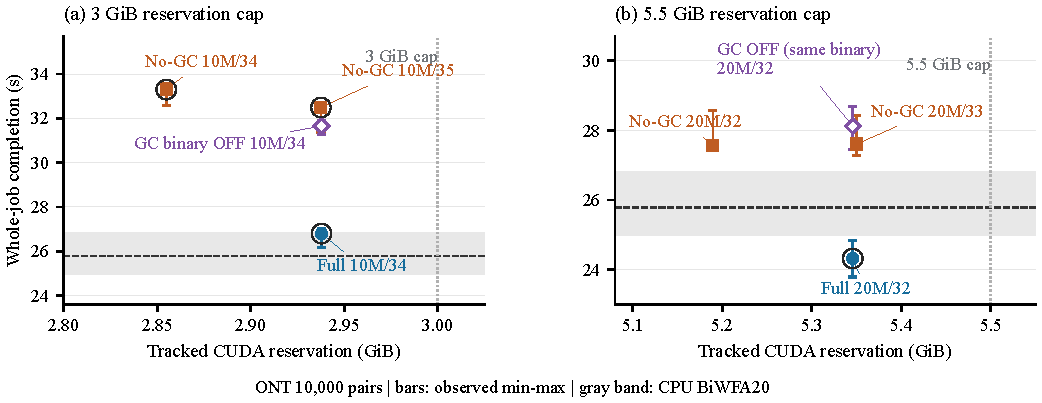
\includegraphics[width=\textwidth]{figures/budget_time.pdf}
\caption{Tracked CUDA reservation versus whole-job completion for revised-source controls. Bars are observed min--max across crossed profiler-off repetitions. The horizontal CPU band is its observed time range, without a GPU-reservation coordinate. Rings mark nondominated measured median points only; no unmeasured operating point is interpolated. The two panels use different horizontal and vertical ranges.}
\label{fig:budget}\end{figure*}

\begin{figure*}[t]\centering
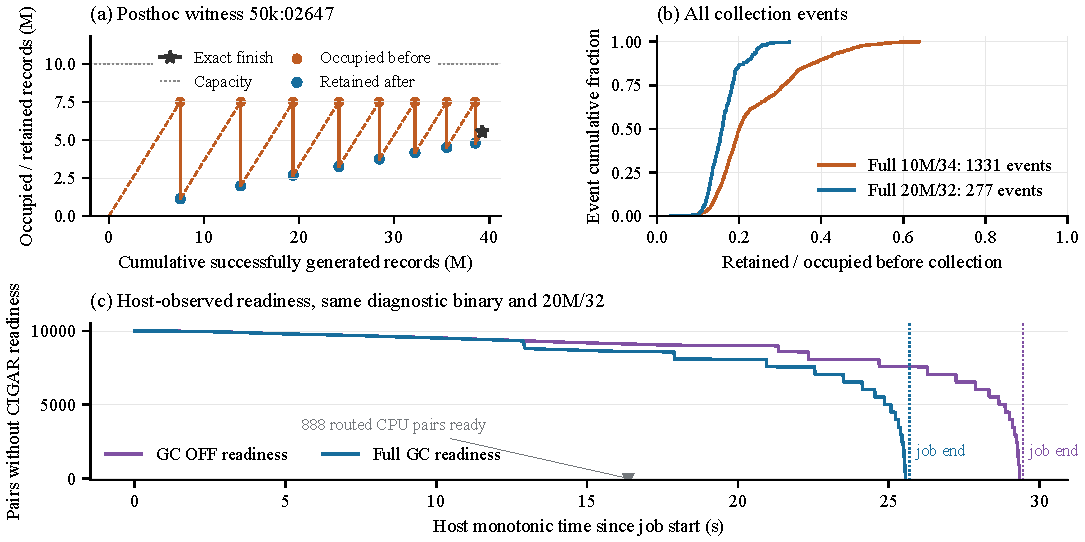
\includegraphics[width=\textwidth]{figures/mechanism.pdf}
\caption{Separate diagnostic evidence. (a) Occupied and retained ancestor-closure records versus cumulative successful generation for an original public pair; M=$2^{20}$ records. Points are collection snapshots; dashed segments only join observed endpoints. (b) Retained/occupied ratios across all Full 10/20 collection events. (c) Host-observed pairs without an alignment/RLE-ready event, including unsupported CPU routing, with matched 20M/32 GC on/off. Host and device clocks remain distinct. Readiness precedes final file close and child exit; these are not primary performance timings.}
\label{fig:mechanism}\end{figure*}

\subsection{Does Small No-GC Recover the Benefit?}
Matched capacity and worker controls answer this directly (Table~\ref{tab:main}). At 10M/34, guarded no-GC rescues \RescueTen{} supported pairs, whereas Full rescues none. At 20M/32 the corresponding counts are \RescueTwenty{} and zero. Both Full settings complete the supported pairs on the GPU and produce valid exact full CIGAR. Thus smaller arena reservation and more workers alone do not explain successful small-arena execution.

The no-GC 10M/35 and 20M/33 controls spend the space saved by omitting GC scratch on an additional worker. They fit the same respective reservation caps and still incur the capacity failures. Figure~\ref{fig:budget} compares revised-source controls; the historical large-arena grid remains separate in the supplement. Relative to the fastest tested lighter guarded configuration under each cap, Full reduces the median by 17.5\% at 3~GiB and 11.8\% at 5.5~GiB. Full's advantage is an operating-configuration result under a cap, not equality of byte allocations or a claim that maximizing workers is always beneficial.


\subsection{Same-Binary Collection On/Off}
At 20M/32 the revised GC binary, with identical allocation in both modes, takes \OffTwenty{}~s with collection off and \FullTwenty{}~s with collection on, a \ModeReductionTwenty{}\% reduction in median whole-job time. Capacity rescues fall from \RescueTwenty{} to zero. The 10M/34 same-binary control also tests the smaller operating point. Holding the binary and scratch constant removes the register/allocation difference from the comparison; it does not isolate a pure collection instruction cost. Collection changes the amount of GPU computation completed, CPU realignment, callback work, overlap and output readiness.

An earlier same-binary experiment observed 28.866 versus 25.191~s (12.7\%) and 118 versus zero rescues. Its six profiler-off runs passed exact validation, but its kernel retained the shared same-value writes fixed in this revision. We preserve that observation as historical evidence, without assuming the hazards cancel or pooling it with the corrected binary. The revised measurements are the primary ablation. The old \texttt{diag\_A} run's external-process STOPPED flag is preserved; that diagnostic is excluded from the revised evidence.

\subsection{What Was Reclaimed?}
Figure~\ref{fig:mechanism} uses separate revised-source diagnostics. The posthoc stress witness \texttt{50k:02647} generates 39.264~M records with 8 collections in a 10M arena; maximum retained closure at those collections is 4.799~M. Occupied records drop at collection boundaries. Retained ancestors, remapped pointers and partial vectors produce a valid optimal full CIGAR. The matching no-GC path instead reaches capacity and realigns on the CPU. The counter identity holds across all successful diagnosed pairs, with no trace overflow. Full 10 and Full 20 each generate 19,939,875,345 records over the eligible input: reclamation changes retention, rather than eliminating those appends.

Across the 20M diagnostic, \CollectedPairsTwenty{} of 9,112 eligible pairs collect, for \CollectionsTwenty{} calls. Retained size and live/occupied ratios are distributions over these collection events, rather than a selected witness alone. The remaining pairs execute no collection. Retained closure is not an ideal algorithm's minimum history; total reclaimed records are cumulative reuse across time, not peak memory returned to CUDA. Collection still pays marking, scan, synchronization, movement and remapping.


\subsection{Why Whole-Job Completion Changes}
Host callback events show where avoided realignment can affect subsequent batch submission. A GPU batch can continue while the host reconstructs or rescues the preceding batch; a long callback can delay later submission. The measured completion trace distinguishes normal RLE reconstruction, CPU rescue and the separately routed 888 pairs. It does not attribute the entire job difference to one last pair or add overlapping phase spans. GC can lengthen GPU work by letting difficult pairs finish while shortening the complete path by avoiding recomputation.

\subsection{Strong Software Alternatives and Applicability}
Smaller $E$ remains exact because it rescues exhausted pairs, but the selection screens increase CPU reprocessing and do not remove the measured tradeoff. The selected $E=8,192$ full-input controls take \SmallEGuard{}~s (guarded) and \SmallEFull{}~s (Full), each with 384 CPU rescues; these are total job times, including rescue. CPU screening confirms feasible med/low/Singletrack outputs and retains \CpuChoice{} for the repeated CPU comparison. High mode fails under the enforced host cap; its signal alone does not prove physical host OOM. These bounded tests do not establish a globally optimal CPU or GPU configuration.

The revised-source short-ONT checks retain the old fixed settings: no-GC 4M/64 uses 2,366.681~MiB and takes 1.455~s, versus Full 2M/64 at 1,374.681~MiB and 1.348~s. Their observed ranges overlap; CPU takes 1.037~s. On the already-seen 2,375-pair CCS confirmation, no-GC 4M/64 takes 3.430~s with 38 rescues, Full 20M/32 takes 2.618~s with zero, and CPU takes 0.569~s. Long length alone does not imply GPU benefit. The post-campaign source-consistency refresh uses three crossed runs per old fixed choice; it neither tunes CCS nor creates a new holdout. A previously unsuccessful selector remains in the supplementary record and is excluded from the method.

\section{Prior Work, Limits, and Conclusion}
WFA supplies score-indexed recurrence \cite{wfa2021}; WFA-GPU supplies persistent workers, compressed traceback and CPU rescue \cite{wfagpu2023}. WFA2 already contains active-root ancestor marking, rank, compaction, remapping and retained prefixes \cite{wfa2lib2026}. Our addition is its qualified block-local execution in fixed GPU worker arenas, independent guarded capacity and measured budget/completion behavior. BiWFA instead uses bidirectional breakpoints and recursive recomputation for exact low-space traceback \cite{biwfa2023}. Singletrack reduces stored affine states and reconstructs limited gap information \cite{singletrack2026}. These are distinct existing techniques; we do not claim a hypothetical unimplemented combination as a baseline.

Khatri et al. already characterize retained footprint, concurrency, CPU memory modes and GPU full-traceback failure envelopes \cite{characterisation2026}. The publisher now verifies its 2026 publication; we inspected the official 29-page supplement and metadata, not the inaccessible complete article. The characterization is motivation and closest context, not evidence of priority for our implementation. Its capacity/concurrency observation is not our novelty claim. A concrete comparison of mechanisms, source locations and untested combinations is provided in Supplementary Material R2.

The scope is one GPU/host, one penalty scheme, finite configurations and an exact global/full-CIGAR contract. No native device OOM is inferred from a software reservation cap. Residency/paging, universal race freedom, arbitrary penalties, prefix-GC qualification, new automatic policies and hardware necessity are unestablished. Root-dependency reasoning, actual-helper tests, independent small DP and public-output checks provide complementary finite evidence; none substitutes for the unavailable sanitizer checks. The prior WSL copy interruption remains an unresolved historical failure, separate from successful runs. No new independent ONT corpus or production arrival trace is claimed.

The practical result is that active-root collection enables useful small-arena GPU execution after matched no-GC alternatives are considered. Measured generation and retained closure explain the reused space; same-binary controls connect it to avoided CPU recomputation and whole-job completion. Strong CPU and negative short/CCS results delimit the operating region. The defensible paper is an implementation and mechanism study, with broader scheduling or architectural claims left for further evidence.

\paragraph{Artifacts} The local companion \href{ICEIC2027_WFA_R2_Research_Package.zip}{\nolinkurl{ICEIC2027_WFA_R2_Research_Package.zip}} contains modified source, receipts and a reproduction guide. The separately delivered \href{Supplementary_Material_R2.pdf}{\emph{Supplementary Material R2}} contains complete settings, failures, proof boundaries and expanded tables. These are named local delivery artifacts; no public repository or DOI is claimed.
\bibliographystyle{IEEEtran}\bibliography{references}
\end{document}
